% !TeX root = ../../../main.tex
\subsection{Introduction}


Time is central to clinical reasoning in critical care.
% ICU p
Patients often follow rapidly evolving trajectories, requiring symptoms, physiologic measurements, treatments, and outcomes to be interpreted relative to admission, deterioration, intervention, and recovery. 
% Sepsis exemplifies this challenge. 
Sepsis trajectories exemplify this challenge.
Although Sepsis-3 remains important for trial eligibility and computational phenotyping \cite{kyriazopoulou2021procalcitonin,ch08:seymour2019derivation}, 
% sepsis is better understood as a heterogeneous clinical trajectory than as a single, uniform state. 
sepsis is better understood as a set of heterogeneous clinical trajectories with a shared dysregulatory response rather than as a single, uniform course. 
Similar temporal challenges extend across critical illness: risk forecasts depend on when evidence becomes available; treatment-response analyses require distinguishing pre- and post-intervention measurements; and retrospective cohort definitions may change when the timing of symptom onset, diagnostic testing, or treatment initiation is misaligned.
This increasing focus on temporal structure is evident in early-warning systems \cite{henry2022factors}, studies showing that predictive utility varies with timing \cite{kamran2024evaluation}, and research on the temporal characteristics of sepsis subtypes and progression \cite{ch08:noroozizadeh2023temporal}.


The growing emphasis on time in critical care reveals an important methodological gap: electronic health records (EHRs) are not organized as temporally grounded patient trajectories. Critical-care repositories such as MIMIC-III/IV \cite{ch08:johnson2016mimic,ch08:johnson2023mimic} make this challenge explicit by combining structured time-series measurements with narrative clinical documentation. These modalities provide complementary but asymmetric evidence for timeline construction (Figure~\ref{ch08:fig:motivation_multimodal_alignment}). Structured rows offer relatively precise temporal information from laboratory results, medications, procedures, vital signs, diagnoses, and administrative events. Clinical narratives, by contrast, provide richer accounts of the patient course, including symptoms, clinician assessments, patient-reported histories, functional status, disease progression, and contextual modifiers. For example, a note describing ``increasing lethargy and peripheral mottling'' may precede an increase in Sequential Organ Failure Assessment (SOFA) scores. Similarly, documented oliguria despite stable creatinine may indicate clinically meaningful states that structured measurements do not fully capture. 

Recent studies point to both the promise and the difficulty of this problem. Multimodal annotation of discharge summaries aligned with structured EHR data demonstrated that access to both modalities can improve the precision of inpatient event timelines, highlighting the value of structured rows as temporal evidence when aligned with the narrative record \cite{ch08:frattallone2024using}. At the same time, text-only timeline reconstruction remains challenging in realistic EHR-style notes, where dense event structure, abbreviations, and semi-structured formatting make both event recovery and time assignment difficult \cite{noroozizadeh2026reconstructing,ch08:noroozizadeh2026forecasting}. Together, these findings motivate more explicit alignment between text-based and tabular approaches, with the goal of improving temporal precision while preserving the richer event content available in narrative text.\cite{ch08:moldwin2021empirical,seinen2025using}

In this work, we investigate whether aligning retrieved structured EHR evidence with text-derived event timelines can improve the temporal precision of reconstructed patient trajectories. Our retrieval-augmented multimodal approach integrates structured rows directly into timeline reconstruction rather than treating textual and tabular data as separate views. The multistep pipeline first identifies temporally informative central events and uses them to create an initial scaffold of the patient trajectory. It then positions additional events relative to this scaffold and refines the resulting timeline using retrieved structured evidence. This decomposition reflects a clinically natural distinction between events that form the backbone of an encounter and those whose timing is best interpreted relative to that backbone. Using this framework, we assess whether and where multimodal alignment improves on text-only timeline reconstruction. Specifically, we examine the effects of introducing structured evidence at different stages of the reconstruction workflow, determine whether improvements are concentrated in temporal metrics rather than event recovery, and analyze which prognostically relevant information appears in text but is missing or delayed in tabular data.

%%%%%%%%%%%%%%%%%%%%%%%%%%%%%%%%%%%%%%%%%%%%%%%%%%

% !TeX root = ../../../main.tex
\begin{figure}[htbp]
\begin{ChEightFloatBody}

    \centering
    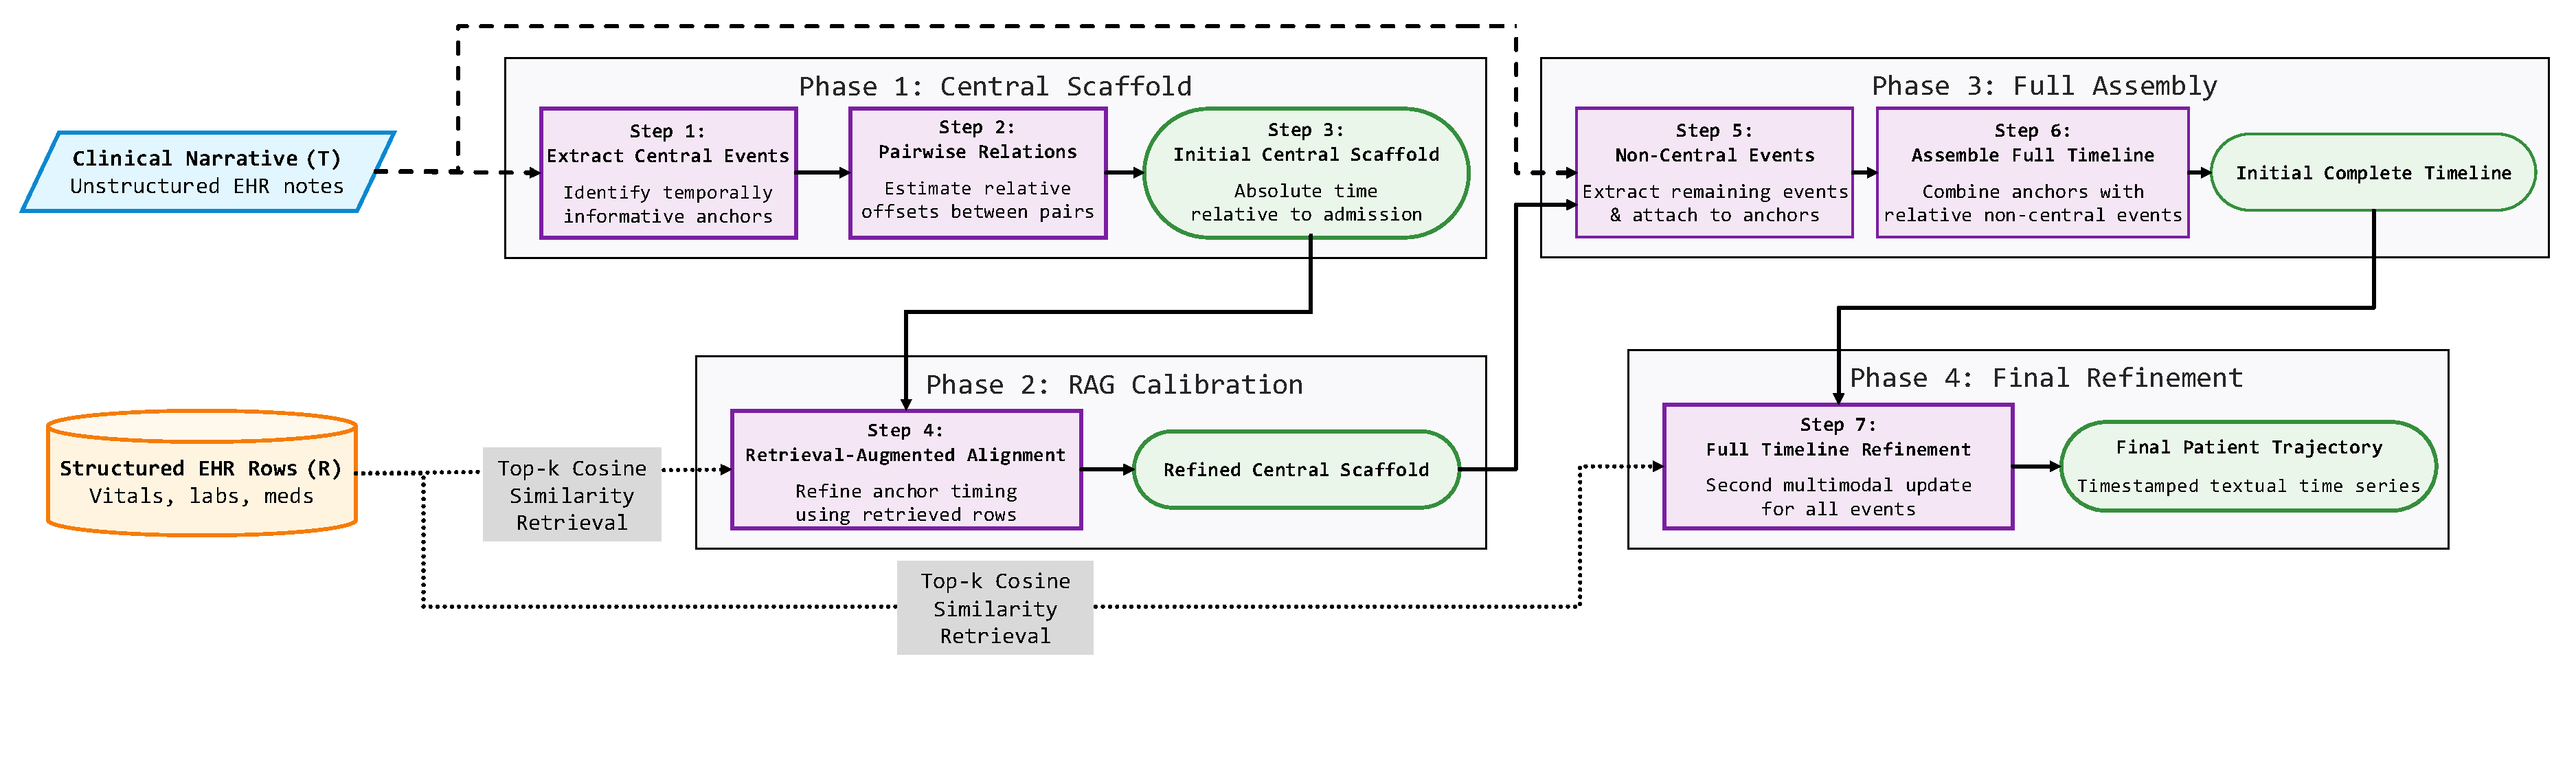
\includegraphics[width=\textwidth]{Chapters/chapter-08/images/plots/TTA-Overview-Figure-Model-Updated.pdf}
    
    
    
    

\end{ChEightFloatBody}
\caption{
    Overview of the scaffolded retrieval-augmented timeline reconstruction workflow. The method first extracts central events from the clinical narrative, estimates pairwise temporal relations, and builds an initial central-event scaffold. Retrieved structured EHR rows are then used to calibrate this scaffold. Non-central events are extracted and attached relative to central events, after which a final retrieval-augmented refinement step calibrates the complete timeline.
    % \textcolor{blue}{Shahriar-update figure to remove symbols if relevant}
    }\ChEightFloatLabel{ch08:fig:pipeline}
\end{figure}

%%%%%%%%%%%%%%%%%%%%%%%%%%%%%%%%%%%%%%%%%%%%%%%%%%

% \vspace{-5pt}
\textbf{Contributions.} In summary, the paper makes the following contributions. \textbf{(i) Temporal grounding formulation:} We formulate clinical timeline reconstruction as retrieval-augmented temporal grounding of narrative-derived patient trajectories using structured EHR evidence. \textbf{(ii) Multimodal scaffolded reconstruction workflow:} We introduce a workflow that uses anchor events as a temporal backbone and retrieved structured rows as partial evidence for timestamp calibration. \textbf{ (iii) Multimodal timeline evaluation:} We evaluate multimodal calibration on 40 discharge summaries with aligned structured EHR rows and manual gold-standard timelines, testing whether structured evidence improves temporal localization more than event recovery. \textbf{(iv) Information missing from tabular data:} We provide an empirical analysis of clinically relevant events that are absent, delayed, or semantically compressed in structured tabular data, motivating why unstructured text is necessary for constructing clinically meaningful patient trajectories.
% \textcolor{blue}{Shahriar - if you can manage space, feel free to add uncertainty analyses and update relevant sections}
%\textcolor{blue}{\textbf{(v) When multimodal alignment helps most:} We characterize performance across event types and timestamp-certainty settings, showing that structured data is especially useful as a temporal calibrator when event timing cannot be directly inferred from text.}

%%%%%%%%%%%%%%%%%%%%%%%%%%%%%%%%%%%%%%%%%%%%%%%%%%
%%%%%%%%%%%%%%%%%%%%%%%%%%%%%%%%%%%%%%%%%%%%%%%%%%

